\chapter{基于多知识库的表格实体链接}

\section{任务描述}\label{2.1}

表格的语义解释的一般任务使用一个表格和一个参考知识库作为输入,通常包括以下三个子任务:

\begin{enumerate}[1.]
\item 实体链接:找到表格单元格中称为 Mention 的文本短语并将其与对应的知识库参考实体相链接
\item 列类型推理:根据表格中一列包含的实体的知识库类型来推断该列的类型
\item 关系抽取:根据两个表中列与列在给定的一行的实体对的关系将来推断列间关系
\end{enumerate}

实体,类型和关系都是来自在给定的知识库中。
举一个具体的例子,给定图~\ref{movie} 中的表格和知识库中文维基百科,实体链接的任务就是将字符串指称 ``冯小刚'' 链接到中文维基百科中的实体\textbf{冯小刚}。
列类型推理的任务就是将表格第二列与中文维基百科中的导演类型相关联。
关系抽取任务则是识别实体\textbf{冯小刚}和\textbf{非诚勿扰}之间的关系\textbf{isDirectorOf}。
在这篇文章中,我专注于第一个语义解释任务,实体链接。
实体链接在自然语言处理 (Natural Language Processing) 领域也叫做命名实体消岐 (Named Entity Disambiguation)。
需要额外说明的是,我做的是中文的实体链接系统,而不是跨语言的实体链接\cite{zhang2013cross}。
接下来会正式定义表格的实体链接任务。
还会介绍文章中的用到的一些符号含义。\newline\par

% Fig 2.1
\begin{figure}[htbp]
\centering
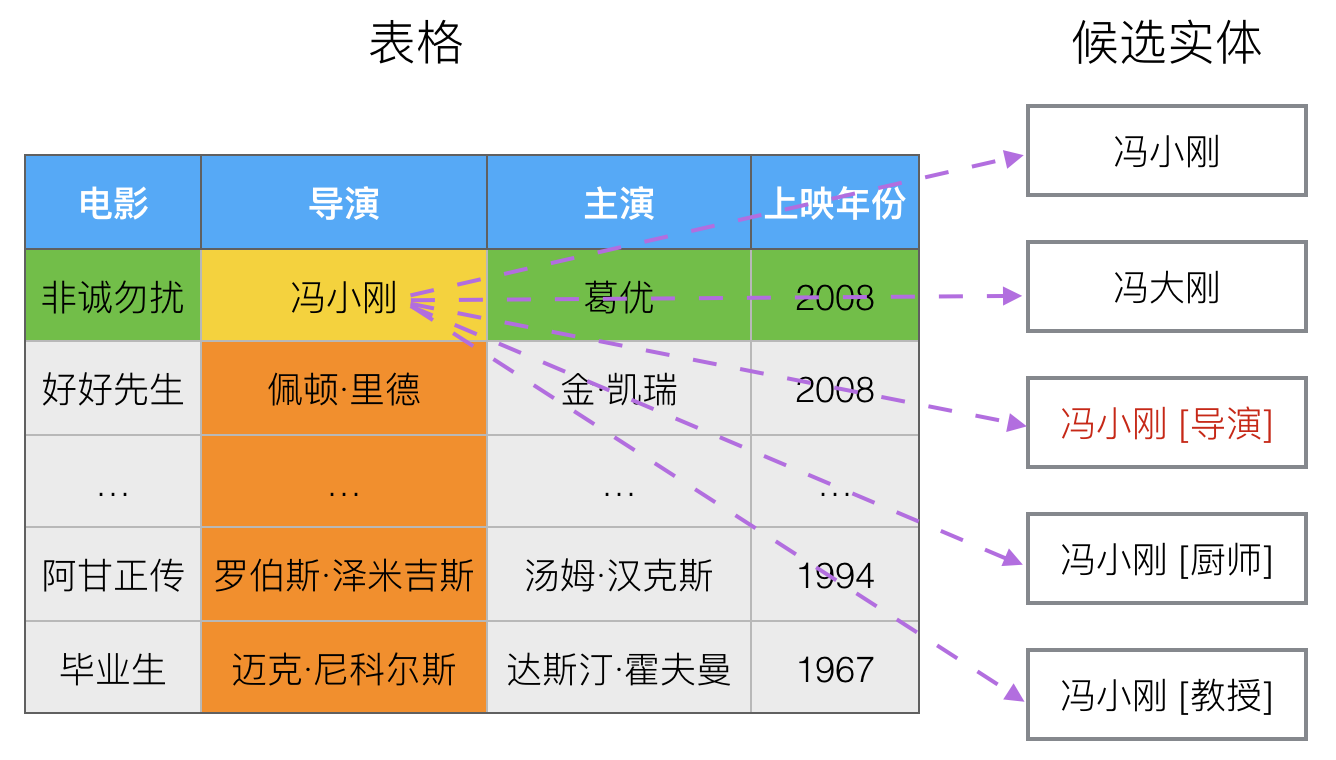
\includegraphics[width=0.9\textwidth]{img/movie}
\caption{一个对于实体链接任务的演示。左边表格中已识别出的字符串指称位于黄色单元格中。正确的链接实体用红色标出。}
\label{movie}
\end{figure}

\noindent\textbf{正式定义}

一个表格在系统中被表示为一个矩阵,$T$,该表格包含 $r$ 行 $c$列。使用行和列单位的表格很容易规范化成 $r\times{c}$ 的矩阵。$T[i,j]$代表了 $T$在 $i^{th}$ 行和 $j^{th}$ 列的单元格。
一个字符串指称 $m$ 指的是表格单元格中的一个字符串,该字符串需要事先被识别出来并且能潜在得指向知识库中的一些实体。
在语义网领域中,实体可以理解为独立存在且相互区别的某种事物,并不一定是物质上的存在,可能是一个词语或者一种概念。比如``迈克尔·乔丹''、``苹果''都是语义网中的实体。
在我的系统中,实体来自最大的中文链接开放知识库 Zhishi.me\cite{niu2011zhishi},其包含了三个相互链接的中文百科型知识库:百度百科、互动百科和中文维基。
有一些表格中字符串指称在给定的知识库中可能不存在对应的实体,这样的无对应实体的指称被称为不可链接的指称 (Unlinkable Mention),在我的系统中会给这样的指称打上一个特殊的标签 ``NIL'' 来表明它是不可链接的。
对于不可链接的指称,现有一些研究\cite{shen2012ontology}\cite{ling2012}会识别它们在知识库中的细粒度类型 (Fine-grained Type),但这个已经超出实体链接系统的范围。\newline

\noindent\textbf{任务:} 给定多个知识库的实体集合 $E$ 和一个表格中字符串指称集合 $M$,多知识库的表格实体链接的目标就是将表格中的每个字符串指称 $m \in M$ 链接到知识库中它的对应参考实体 $e \in E$。


\section{关键挑战}

现在对实体链接的研究开展得如火如荼,研究者们提出了大量的前景广阔的技术,从深度神经网络到联合推理方法。
但是很多论文都没有提及或者思考过实体链接中可能遇到的各项挑战或困难。
而这些关键挑战可能会对实体链接的效果产生很大的影响。
在实现表格实体链接系统的过程中以及在完成各项对比试验的过程中,我遇到了许多挑战与困难。
接下来我会将它们一一罗列出来,希望在未来的工作中能够战胜这些挑战。\par

\begin{enumerate}[1.]
\item \textbf{缺乏基准数据集} \newline
在实体链接的各项研究中,一个标准化的基准 (Benchmark) 是非常重要的。
这个基准包含3个部分:数据集,知识库和算法的评价标准。
在大多数研究中,知识库普遍会选取维基百科,算法的评价标准基本上差不多。
因此在这里,缺乏基准主要是指缺乏一个标准的高质量的数据集。
在英文领域,有一些常用的数据集可用于实体链接算法的训练和测试。
比如 UIUC 的 ACE 和 MSNBC 数据集,AIDA 研究组的数据集以及 TAC-KBP 研究组的数据集。
但是在中文领域,公开的高质量的实体链接数据集很稀有。
这样就导致了研究者在进行实体链接研究之前,需要自己耗费很多时间精力去准备数据集。
每个人制作的数据集都是不同的,这也导致了在比较不同研究中的算法性能时的很多困难。
在我的实验中,所有的数据集,也就是 Web 表格,都是从 Web 上人工精心挑选出来的。
确保每个表格中的数据准确无误,同时表格中带有许多有歧义的字符串指称,只有这样才能有效地验证算法的消岐性能。

\item \textbf{自然语言的多样性和歧义性} \newline
自然语言在表达上常常带有多样性和歧义性。
多样性指的是一义多词,同一意义可以以多种不同的方式表达,同一个知识库实体被多个字符串指称表示。
歧义性指的是一词多义,同一个词在不同的上下文中有多种不同的意义,同一个字符串指称可以表示多个不同的实体。
自然语言的这2个特性都对实体链接带来了一定的挑战,尤其是歧义性。
例如,对于字符串指称``小米'',如果其上下文为``小明喜欢喝小米粥而不是皮蛋瘦肉粥'',那么它表示的是粮食类实体``小米'';
如果它出现在这样的上下文中,``小米手机真的太酷了'',此时它代表的是手机品牌类实体``小米''。
如果实体链接算法不能很好的理解字符串指称的上下文,那么很有可能链接到的就是一个错误的实体。
所以,字符串指称的上下文特征在一些实体链接算法中是相当重要的,能否抽取出高质量的字符串指称上下文特征决定了能否对字符串指称进行正确的消岐。

\item \textbf{实体缺失} \newline
就像~\ref{2.1} 节中提到的,知识库中的实体数量有限,不可能覆盖世界上的所有实体。
因此,在实体链接的过程中,肯定会遇到一些字符串指称没有候选实体,链接不到任何一个知识库实体的情况。
这就是实体缺失的问题。在我看来,解决实体缺失最好的办法就是不断扩大知识库的规模,尽可能让它拥有更多实体。
现在很多知识库还是依赖于人工撰写页面的方式来收录知识,知识库规模扩大的速度可能永远跟不上 Web 上信息增长的速度,因此实体缺失的问题可能会长期存在。
对于``不可链接 (unlinkable)''的字符串指称,一些研究者\cite{zhang2013zhishilink}\cite{dredze2010entity}直接给这样的实体打上一个``NIL''标签,表示该字符串指称不代表任何实体。
预测不可链接实体是实体链接系统的一个重要模块。
在我的系统中,为了预测哪些字符串指称是不可链接的,使用了一个简单的启发式的方法,那就是如果一个字符串指称 $m$ 的候选实体集合 $E_m$ 是空集,那么就认为该指称 $m$ 是不可链接的并返回一个 NIL 标签给它。
除此之外,还有许多预测不可链接实体的方法,在本文中就不再赘述。


\end{enumerate}


\section{链接流程}

对于一个一般的表格实体链接系统,给定一个表格和一个知识库的实体,系统执行实体链接任务主要分为三步:

\begin{enumerate}[1.]
\item 指称识别 (Mention Identification):在表格单元格中识别出每个潜在的指称。
\item 候选实体生成 (Candidate Generation):对于每个潜在的指称,生成其候选实体集合,知识库中的实体子集都可能是潜在指称的参考实体。
\item 实体消岐 (Entity Disambiguation):对于每个潜在的指称,根据指称的上下文从其候选实体集合中挑选出一个实体作为字符串指称的参考实体。
\end{enumerate}

我的毕设系统中的2个方法基本都遵循这三个步骤,不同之处在于系统的输入变成了多个知识库的实体以及在实体消岐算法部分有一些区别。
系统使用的是监督学习的方法,我事先人工标注了表格数据集并使用已标注的指称来训练系统的各个模块。
尽管我在实验中使用百度百科、互动百科和中文维基百科作为实验的知识库,但我的方法是通用的,只要给定任意一个知识库中的已标注数据,便可使用该知识库。
关于系统中2个多知识库实体链接方法的步骤和细节会在第三章中详细介绍。

% Fig 2.2
\begin{figure}[htbp]
\centering
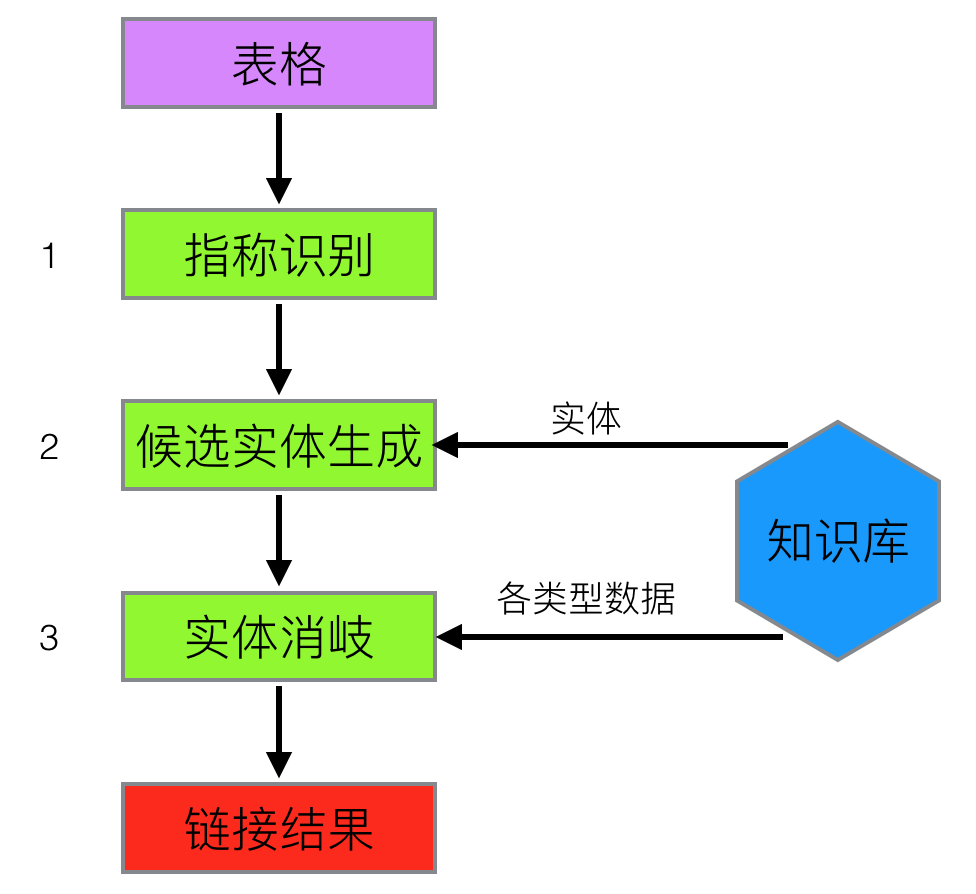
\includegraphics[width=0.6\textwidth]{img/flow}
\caption{实体链接的一般流程}
\label{flow}
\end{figure}


\section{本章小结}
本章是对多知识库表格实体链接所需的背景知识的一个梗概介绍。
先描述了表格语义解释的3个子任务,明确了多知识库表格实体链接这个任务的定义,如图~\ref{movie} 所示。
然后讲述了一些实体链接过程中的关键性挑战,包括我在实验过程中遇到的困难。
最后介绍了表格实体链接的一般流程,如图~\ref{flow} 所示。
在下一章中我会详细得讲述我的毕设系统的设计思路和各模块组成,尤其是2个多知识库表格实体链接方法的步骤和异同。





